\section{排序與搜尋}

    \subsection{排序}
    \author{ShangJhe Li}
    排序就是將所有的資料重新整理,方便後面搜索使用。許多演算法都是建立在排序上,例如二分搜尋法就是其中之一。

    排序有很多種,最常見的就是合併排序、快速排序。詳細的排序演算法可以參考其他網站。

    在程式競賽上,如果你使用C++,則我們可以直接利用 \verb|sort()| 函式將所有東西排好。(但還是建議上述兩個演算法要學會)

    一般情況下, \verb|sort| 都會用 \verb|less<T>| 來排序,也就是由小到大。因此我們只需要給他你要排序的起點終點就可以了。

\begin{lstlisting}[caption=一般的sort]
int n,a[100];
sort(a,a+n);
vector<int> b;
sort(b.begin(),b.end());

\end{lstlisting}
        
    但如果你希望他由大到小,我們有許多方式可以用。

\begin{lstlisting}[caption=由大到小排]
int n,a[100];
sort(a,a+n,greater<int>());

// 使用比較函式
bool cmp(int a,int b){
    return a>b;
}
vector<int> b;
sort(b.begin(),b.end(),cmp);

// 使用lambda function(較快)
sort(b.begin(),b.end(),[](int a,int b){
    return a>b;
});

// 使用函數物件(較快)
struct cmp{
    bool operator()(int a,int b){
        return a>b;
    }
}
sort(b.begin(),b.end(),cmp);

\end{lstlisting}

    眼尖的你或許有發現可以利用後面三種方法,完成各種方式的排序。

    沒有錯,這就是為什麼我們暫時不需要學習自己寫演算法。

    \example 第一屆卓越盃 C.Safe Sorter

    我們的保險箱現在要放到一個分類器之中,此分類器有許多節點(如下圖),放入的規則如下。

    \begin{figure}[h]
        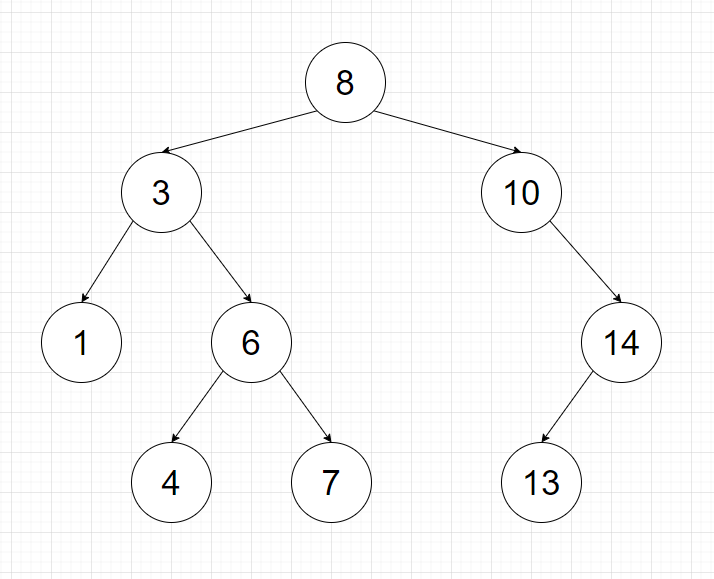
\includegraphics[width=\textwidth]{../Images/SaveSorter.png}
    \end{figure}

    \begin{itemize}
        \item 如果該節點還沒有任何保險箱,此保險箱就會佔據該節點
        \item 否則若這個要放入的保險箱裡面的金塊比在該節點的保險箱還要多,他會被往右邊送
        \item 否則就往左邊送
        \item 必須送到他占用一個節點為止
    \end{itemize}

    以下圖為例

    \begin{itemize}
        \item 第一個放進來的保險箱有 8 個金塊
        \item 第二個有 10 個,因此他被放在右邊
        \item 第三個有 14 個,因此第一步會先往右送,發現右邊的節點也有保險箱了,因而再次被往右送
        \item 第四個有 3 個,於是被放在左邊
        \item 其他依此類推
    \end{itemize}

    由於分類器內部構造太大,不方便進入,所以開發者在分類器中內建一套電梯探訪順序,以及記錄規則供使用者參考,避免保險箱被重複計算或是漏算。如下

    \begin{itemize}
        \item 當此節點的左邊有保險箱,電梯優先向左
        \item 當此節點的左邊的保險箱都被記錄過了,或是左邊根本沒有保險箱,紀錄當前所在的節點裡面保險箱的金條數量
        \item 然後電梯向右
    \end{itemize}

    同樣以上圖為例

    \begin{itemize}
        \item 節點 8 的左邊有其他保險箱 >> 電梯向左
        \item 進到節點 3 >> 同上 >> 電梯向左
        \item 進到節點 1 >> 左右邊都沒有保險箱 >> 記下 1 >> 電梯回到節點 3
        \item 左邊都記錄過了 >> 記下 3 >> 右邊有保險箱 >> 電梯向右
        \item 進到節點 6 >> 左邊有其他保險箱 >> 電梯向左
        \item 進到節點 4 >> 左右邊都沒有保險箱 >> 記下 4 >> 電梯回到節點 6
        \item 左邊都記錄過了 >> 記下 6 >> 右邊有保險箱 >> 電梯向右
        \item 進到節點 7 >> 左右邊都沒有保險箱 >> 記下 7 >> 電梯回到節點 6
        \item 電梯回到節點 3 >> 電梯回到節點 8 >> 左邊保險箱紀錄完畢 >> 記下 8 >> 右邊有保險箱 >> 電梯向右
        \item 進到節點 10 >> 左邊沒有保險箱 >> 記下 10 >> 右邊有保險箱 >> 電梯向右
        \item 進到節點 14 >> 左邊有保險箱 >> 電梯向左
        \item 進到節點 13 >> 左右邊都沒有保險箱 >> 記下 13 >> 電梯回到節點 14
        \item 左邊保險箱紀錄完畢 >> 記下 14
        \item 電梯回到節點 10 >> 電梯回到節點 8
        \item 紀錄完畢
    \end{itemize}

    最後結果如下

    \verb|1 3 4 6 7 8 10 13 14|

    \textbf{輸入說明}

    \begin{itemize}
        \item 第一行輸入 $1$ 個數字 $t$ ,代表有 $t$ 比測試資料
        \item 每筆測資第一行輸入 $1$ 個數字 $n$ ,表示一開始的保險箱有幾個
        \item 第二行輸入 $n$ 個數字 $a_1,a_2...a_n$ , $a_i$ 代表第 $i$ 個放入分類器的保險箱有幾塊金條
    \end{itemize}

    $t \leq 10$ $,$ $n$ $,$ $a_i$ $\leq 10^5$

    \textbf{輸出說明}

    僅全部的保險箱放完以後進行一次紀錄
    
    \begin{tabular}{|m{7cm}|m{7cm}|}
        \hline
        範例輸入 1 & 範例輸出 1 \\
        \hline
        \verb|2|        &  \verb|1 2 3| \\
        \verb|3|        &  \verb|1 3 4 6 7 8 10 13 14| \\
        \verb|3 2 1|
        \verb|9|  
        \verb|8 10 14 3 1 6 7 4 13|\\
        \hline
        範例輸入 2 & 範例輸出 2 \\
        \hline
        \verb|18| &  \verb|9| \\
        \hline
    \end{tabular}

    \textbf{子題組與配分}

    \begin{itemize}
        \item 第一子題組 : 放入的順序為由大到小,占 $10\%$
        \item 第二子題組 : 無其他限制,占 $90\%$
    \end{itemize}

    仔細閱讀題目後我們可以發現,經過複雜的操作後,輸出值恰為由小到大排序的數列。所以我們就可以使用\verb|sort()|解決。

    \subsection{線性搜尋}

    說實話,線性搜尋就是暴力而已,直接放上程式碼。

\begin{lstlisting}[caption=線性搜尋]
int finding(vector<int> &v,int target){
    for(int i=0;i<v.size();++i){
        if(v[i]==target){
            return i;
        }
    }
    return -1;
}
\end{lstlisting}

    當然,我們可以在if裡面放入其他有趣的判斷式。這也是我仍然有放這個單元的原因。

    \subsection{二分搜尋}
    \textbf{Author:李卓岳}
    \author{李卓岳}

    二分搜能運用到的場合相當多,只要是\textbf{單調區間}便可使用二分查找,主要的題目類型有:

    \begin{itemize}
        \item 尋找特定值
        \item 查找第一個大於等於某數的元素
        \item 查找最後一個小於等於某數的元素
        \item ...
    \end{itemize}

    二分搜說難也難、說簡單也簡單,主要是實作過程中有\textbf{許多細節}需要注意:

    \begin{itemize}
        \item $left, right$要初始為$(0,n-1)$還是$(0,n)$?
        \item $while$判斷式中要填$left<=right$還是$left<right$?
        \item 更新$left$和$right$時$mid$要$+1$還是$-1$?
    \end{itemize}    

    就這些細節可知二分搜有許多類型和細節,為求解題方便以下將提出一套思路使你在面對各類型的題目時,都能輕易找出對應的寫法。

    \subsubsection{實作}

    \example 大於等於
    
    \textbf{問題定義}

    給定一\textbf{單調上升之數列},求第一個\textbf{大於等於某特定值}的元素索引值並定義其為「下界」,當下界不存在則回傳數組長度。

    \textbf{思路}

    給定數組\verb|[1,2,4,5,5,6,7]|,令特定值為$5$則應該回傳下界為$3$。

    \begin{center}
    \begin{tabular}{|c|c|c|c|c|c|c|}
        \hline
        0 & 1 & 2 & $\to$3 & 4 & 5 & 6 \\
        \hline
        1 & 2 & 4 & $\to$5 & 5 & 6 & 7 \\
        \hline
    \end{tabular}
    \end{center}
    
    可以看到我們能將數列分為\textbf{右側都大於等於特定值}和\textbf{左側都小於特定值},而我們回傳之索引值正好是\textbf{大於等於特定值的數列之下界}。

    首先,我們以\textbf{閉區間}之寫法來表達思路:

    \begin{itemize}
        \item 區間範圍為$[left,right]$,$left$指向索引值$0$,$right$指向索引值$6$
        \item $mid$為$[left,right]$的中間位置
        \item \textbf{當$left>right$時,區間為空}
    \end{itemize}

    依據上述思路提出,演算法步驟:

    \begin{enumerate}
        \item 若$arr[mid]>=$特定值,則$[mid,right]$區間內所有元素均大於等於特定值,因此right左移,故\textbf{$right=mid-1$}。
        \item 否則,則是$[left,mid]$區間內所有元素均小於特定值,因此$left$右移,故\textbf{$left=mid+1$}。
        \item 重複上述動作直到區間被刪減為空,\textbf{此時$left$將會停在下界,故回傳$left$}。
    \end{enumerate}

    \textbf{程式碼}

    可執行下列程式碼以利思考。

    \begin{lstlisting}
#include<bits/stdc++.h>
#define ll long long
using namespace std;
int a[100005];
int main(){
    int n,x;
    
    cin>>n;
    for(int i=0;i<n;++i)cin>>a[i];
    cin>>x;
    sort(a,a+n);
    
    int left=0,right=n-1;//[0~N-1]的閉區間 
    while(left<=right){//[left~right]大小為零結束 
        int mid=(right+left)/2;
        //cout<<left<<' '<<mid<<' '<<right<<'\n';
        if(a[mid]>=x) right=mid-1;
        else left=mid+1;
    }
    
    cout<<left<<'\n';//回傳索引值
    return 0;
}\end{lstlisting}
    
    \example 小於等於

    \textbf{問題定義}

    給定一\textbf{單調上升之數列},求最後一個\textbf{小於等於某特定值}的元素索引值並定義其為「上界」。

    \textbf{思路}

    給定數組\verb|[1,2,4,5,5,6,7]|,令特定值為$5$則應該回傳下界為$3$。

    \begin{center}
    \begin{tabular}{|c|c|c|c|c|c|c|}
        \hline
        0 & 1 & 2 & 3 & $\to$4 & 5 & 6 \\
        \hline
        1 & 2 & 4 & 5 & $\to$5 & 6 & 7 \\
        \hline
    \end{tabular}
    \end{center}

    首先我們一樣能將數列分為右側都大於特定值和左側都小於等於特定值,透過觀察我們可以發現,\textbf{小於等於特定值的數列上界和大於特定值下界是相鄰的}所以\textbf{上界 $=$ 下界 $- 1$}。因此,所有找上界的問題,都可以\textbf{轉換為「互補的」找下界的問題}。

    \begin{itemize}
        \item 區間範圍為$[left,right]$,$left$指向索引值$0$,$right$指向索引值$6$
        \item $mid$為$[left,right]$的中間位置
        \item \textbf{當$left>right$時,區間為空}
        \item 這次要查找的元素為大於特定值,故\textbf{$right$判斷式要改為$a[mid]>x$}
    \end{itemize}

    依據之前的思路提出相同的演算法步驟:
    \begin{enumerate}
        \item 若$arr[mid]>=$特定值,則$[mid,right]$區間內所有元素均大於等於特定值,因此right左移,故\textbf{$right=mid-1$}。
        \item 否則,則是$[left,mid]$區間內所有元素均小於特定值,因此$left$右移,故\textbf{$left=mid+1$}。
        \item 重複上述動作直到區間被刪減為空,\textbf{此時$left$將會停在下界而$right$會停在$left-1$的位置即為「上界」,故回傳$right$}。
    \end{enumerate}

    \begin{lstlisting}
#include<bits/stdc++.h>
#define ll long long
using namespace std;
int a[100005];
int main(){
    int n,x;
    
    cin>>n;
    for(int i=0;i<n;++i)cin>>a[i];
    cin>>x;
    sort(a,a+n);
    
    int left=0,right=n-1;//[0~N-1]的閉區間 
    while(left<=right){//[left~right]大小為零結束 
        int mid=(right+left)/2;
        //cout<<left<<' '<<mid<<' '<<right<<'\n';
        if(a[mid]>x) right=mid-1;
        else left=mid+1;
    }
    
    cout<<right<<'\n';//回傳索引值
    return 0;
} \end{lstlisting}

    \subsubsection{總結}
    二分搜無論是找下界、還是找上界,都可以套用「找下界」的思路來實作。

    \subsubsection{C++二分搜函式}
    
    $1.$ \verb|lower_bound(begin,end,num,greater())|
    
    從陣列的$begin$位置到$end-1$位置二分查詢第一個小於或等於$num$的數字,找到返回該數字的地址,不存在則返回$end$。 

    \begin{lstlisting}
#include<bits/stdc++.h>
#define ll long long
using namespace std;
int a[100005];
int main(){
    int n,x;
    cin>>n;
    for(int i=0;i<n;++i)cin>>a[i];
    cin>>x;
    cout<<lower_bound(a,a+n,x)-a<<'\n';
    // 通過返回的地址減去起始地址begin,得到索引值
    return 0;
} \end{lstlisting}

    $2.$ \verb|upper_bound(begin,end,num,greater())|
    
    從陣列的$begin$位置到$end-1$位置二分查詢第一個小於$num$的數字,找到返回該數字的地址,不存在則返回$end$。

    \begin{lstlisting}
#include<bits/stdc++.h>
#define ll long long
using namespace std;
int a[100005];
int main(){
    int n,x;
    cin>>n;
    for(int i=0;i<n;++i)cin>>a[i];
    cin>>x;
    cout<<upper_bound(a,a+n,x)-a<<'\n';
    //通過返回的地址減去起始地址begin,得到索引值
    return 0;
} \end{lstlisting}

    $3.$ \verb|binary_search(begin,end,num,greater())|
    
    從陣列的$begin$位置到$end-1$位置二分查詢$num$是否存在陣列中,找到返回$True$,不存在則返回$False$。

    \begin{lstlisting}
#include<bits/stdc++.h>
#define ll long long
using namespace std;
int a[100005];
int main(){
    int n,x;
    cin>>n;
    for(int i=0;i<n;++i) cin>>a[i];
    cin>>x;
    cout<<upper_bound(a,a+n,x)-a<<'\n';
    // 通過返回的地址減去起始地址begin,得到索引值
    return 0;
} \end{lstlisting}

    \subsection{範例與練習}
    \problem 暴力之美

    \textbf{題目敘述}

    給你一個陣列,請幫我找到一個數字是比$m$大的最小值。

    \textbf{輸入說明}

    第一行有兩個正整數$n, m$
    接下來一行有$n$個正整數。

    $n \le 10^7$

    \textbf{範例測試}

    \begin{tabular}{|m{7cm}|m{7cm}|}
        \hline
        範例輸入 1 & 範例輸出 1 \\
        \hline
        \verb|5 3|       &  \verb|5| \\
        \verb|6 3 7 5 1| &  \\
        \hline
        範例輸入 2 & 範例輸出 2 \\
        \hline
        \verb|10 3|                &  \verb|4| \\
        \verb|5 3 7 5 1 7 5 3 8 4| &  \\
        \hline
    \end{tabular}

    \begin{tip}
        二分搜反而不會過呢!想想為什麼。沒有錯,因為這時候的$\log(n)$可是有$20$多喔!
    \end{tip}

    \problem \verb|APCS_2022/1| 4.牆上海報

    \textbf{題目敘述}

    有一個由$n$個木板所組成的柵欄,每個木板的高度為$h_1, h_2, \cdots , h_n$,有$k$張海報要張貼在柵欄上,每張海報的寬度為$w_1, w_2, \cdots w_k$並且高度均為$1$。
    若要張貼海報在高度為$x$的高度,則第$i$張海報需要張貼在一個長度為$w_i$的連續並且高度都不小於$x$的木板上,且每張海報張貼的高度需要一致、按照順序並不能重疊(可以相連)。詢問最高可以貼到多高的位置。

    \textbf{輸入說明}

    第一行有兩個正整數$n, k$
    接下來一行有$n$個正整數代表每個木板的高度
    最後一行有$k$個正整數代表每張海報的寬度。

    $n \le 2 \times 10^5$,$k \le 5000$,$h_i \le 10^9$,$\sum{w_i} \le n$

    \textbf{輸出說明}
    
    輸出共 1 行,包含 1 個整數,代表最大高度。

    \textbf{範例測試}

    \begin{tabular}{|m{7cm}|m{7cm}|}
        \hline
        範例輸入 1 & 範例輸出 1 \\
        \hline
        \verb|5 1|       &  \verb|3| \\
        \verb|6 3 7 5 1| &  \\
        \verb|3|         &  \\
        \hline
        範例輸入 2 & 範例輸出 2 \\
        \hline
        \verb|10 3|                &  \verb|5| \\
        \verb|5 3 7 5 1 7 5 3 8 4| &  \\
        \verb|2 2 1| &  \\
        \hline
    \end{tabular}